% The most comprehensible way of showing your final design 
% (and why it matters) is to give a walkthrough of the key task.
%
% make a sequence of screenshots. Crop and add callouts if necessary 
% to reveal detail such as text in the UI.
%
% Start by showing the final design, then explain why you did it
% 
% keep intro and walkthrough short by explaining only 
% (this is not literature class. Don’t give in to “but if I say 
% everything right away, why would attendees/readers continue to 
% pay attention?”

\subsection{Walkthrough}

One of the most widely used features of social websites is picture browsing 
and having a good laugh about other peoples ugliness.
That's why we provide corresponding functionality to perform this task.
%
\begin{figure}[h]
  \begin{center}
    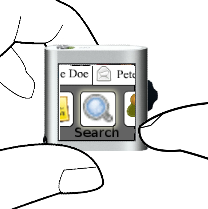
\includegraphics[width=0.6\linewidth]{imgs/wt1.png}
  \end{center}
  \caption{The Main Screen with Vertical Scrolling, Thumb-sized Icons}
  \label{fig:main}
\end{figure}
%
\ldots
%
\begin{figure}[h]
  \begin{center}
    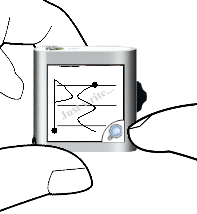
\includegraphics[width=0.6\linewidth]{imgs/wt2.png}
  \end{center}
  \caption{The Writing Recognition Offers Visual Feedback}
  \label{fig:main}
\end{figure}
%
\ldots
%
\begin{figure}[h]
  \begin{center}
    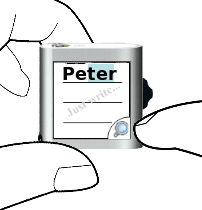
\includegraphics[width=0.6\linewidth]{imgs/wt3.png}
  \end{center}
  \caption{Type-Ahead for Quick Access}
  \label{fig:main}
\end{figure}
%
\ldots
%
\begin{figure}[h]
  \begin{center}
    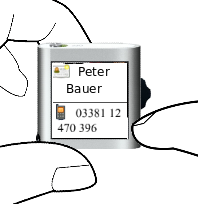
\includegraphics[width=0.6\linewidth]{imgs/wt4.png}
  \end{center}
  \caption{A Vertically Scrolling Profile View}
  \label{fig:main}
\end{figure}
%
\ldots
%
\begin{figure}[h]
  \begin{center}
    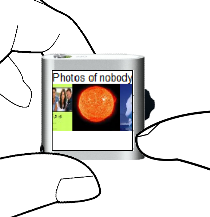
\includegraphics[width=0.6\linewidth]{imgs/wt5.png}
  \end{center}
  \caption{Viewing Albums of a User}
  \label{fig:main}
\end{figure}
%
\ldots
%
\begin{figure}[h]
  \begin{center}
    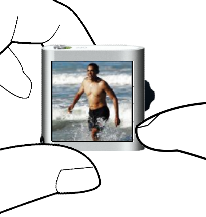
\includegraphics[width=0.6\linewidth]{imgs/wt6.png}
  \end{center}
  \caption{A Fullscreen Photo View}
  \label{fig:main}
\end{figure}
%
\ldots
%
